%\documentclass[10pt,a4paper]{article}
\documentclass[10pt,a4paper]{scrreprt}
\usepackage[utf8]{inputenc}
\usepackage{amsmath}
\usepackage{amsfonts}
\usepackage{amssymb}
\usepackage{graphicx}
\usepackage[left=2cm,right=2cm,top=2cm,bottom=2cm]{geometry}
\usepackage{natbib}
\usepackage{bm}

\usepackage{pythonhighlight}

% integral d
\newcommand{\myd}{\;\mathrm{d}}
% overbar
\newcommand{\overbar}[1]{\mkern 1.5mu\overline{\mkern-1.5mu#1\mkern-1.5mu}\mkern 1.5mu}

\author{Yi Hu}
\title{Homogenization for Multi Field Modelling}
\subtitle{Part I: Theories and FEniCS}

\begin{document}

\chapter{Finite Element Framework FEniCS}

FEniCS project was started at University of Chicago and Charmers University of Technology in 2003. The name ``FEniCS" consists ``FE", ``Finite Element" and ``CS", ``Computational Software". ``ni" makes the name sound like ``phenix". It is a collection of packages that make the best of each package to realize Computational Mathematical and Modelling. The main interface language of FEniCS is Python, which is a fast language for prototyping, while the most of codes and libraries are implemented in C++, whose efficiency in computing stands out. Various linear algebra backends and parallelization allow FEniCS boost in speed. As for modelling, UFL (Unified Form Language) and FFC (FEniCS Form Compiler) allow the direct translation of mathematical formulation such as linear form and bilinear form into symbolic codes. It can be regarded as the language of modelling, which simplifies the modelling process to a large extent \citep{kirby2006compiler}.

This part concentrates on the introduction of FEniCS. Firstly the work flow and components of FEniCS will be presented. Then the most simple example is given in order to clarify its efficiency in modelling. At last some key features of FEniCS is listed and discussed, which provides the flexibility in simulations.

%--------------------------------
\section{The Structure of FEniCS}
The work flow of FEniCS can be described with the following diagram. It is seen that the whole process is decomposed into three major parts. Each part represents one or several functionalities. For form compiler UFL language is involved. With the help of form compiler (FFC), C++ code of the whole model is obtained. Till this point the mathematical derivation, which is the weak form of a PDE in most cases, is converted into pure symbolic efficient C++ codes. The interface between symbolic codes and numerical codes is called UFC (Unified Form-assembly Code). It works as a fixed interface that achieve efficient assembling of finite elements \citep{wells2012automated}.

\begin{figure}[h]
\center
\label{fig: fenics blocks}
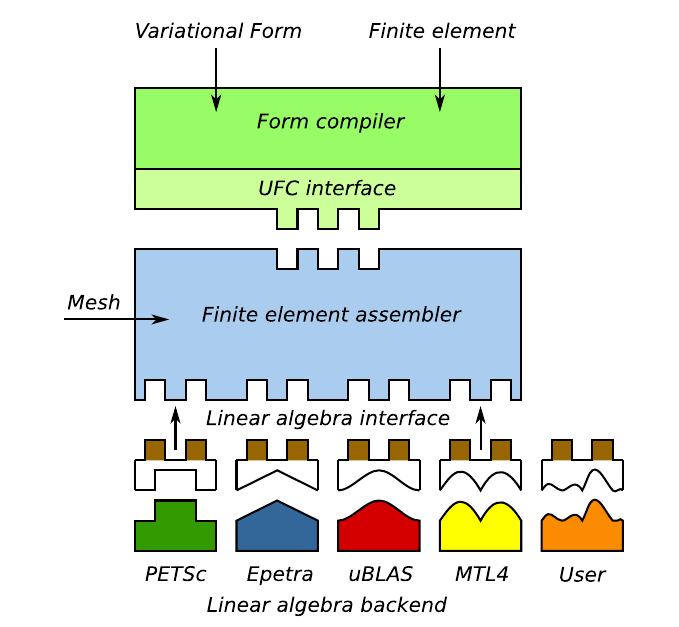
\includegraphics[width=0.6\linewidth]{../pics/fenics_building_blocks.png}
\caption{Building Blocks of FEniCS \citep{wells2012automated}}
\end{figure} 

Numerical algorithms enter after the UFC interface. The main package that carries the numerical algorithm is DOLFIN. DOLFIN's task is to wrap functionalities of each components and their interactions. The user interface of DOLFIN is Python, where object oriented programming can be followed in a easy fashion.  

Other building blocks such as mshr for geometrical modelling and mesh generation, and FIAT (FInite element Automatic Tabulator) for automatic finite element generation for arbitrary orders. Linear algebra backends work as add-ons for FEniCS, which provides the possibility of extension. The visualization package in use is VTK, a substitute of the old one, Viper. The output files could be in various formats. Therefore software like ParaView could apply in terms of visualization. The full structure of FEniCS can be viewed in the following diagram.

\begin{figure}[h]
\center
\label{fig: fenics map}
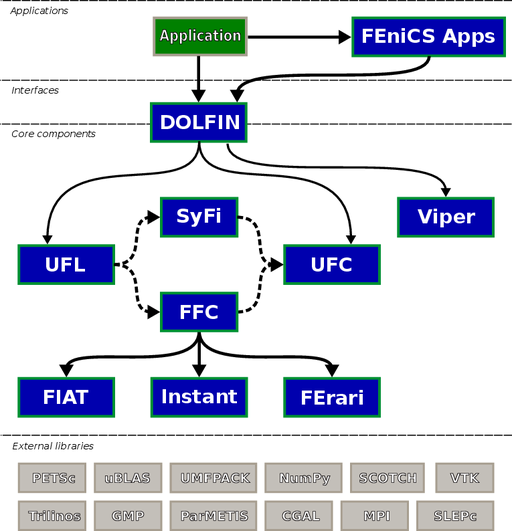
\includegraphics[width=0.5\linewidth]{../pics/fenics_map.png}
\caption{Components of FEniCS \citep{wells2012automated}}
\end{figure} 

%--------------------------------
\section{Simple Poisson Problem}
An implementation of simple Poisson problem is presented in the official tutorial of FEniCS. This example is reproduced here to give a quick overview of the usage and convince its simplicity in modelling \citep{wells2012automated}.

\begin{python}
from dolfin import *

# Create mesh and define function space
mesh = UnitSquareMesh(6, 4)
V = FunctionSpace(mesh, 'Lagrange', 1)

# Define boundary conditions
# Value function for boundary condition x[0]->x, x[1]->y
u0 = Expression('1 + x[0]*x[0] + 2*x[1]*x[1]')
# Mark boundary
def u0_boundary(x, on_boundary):
    return on_boundary
# Add Dirichlet boundary condition
bc = DirichletBC(V, u0, u0_boundary)

# Define variational problem
u = TrialFunction(V)
v = TestFunction(V)
f = Constant(-6.0)
# Bilinear Form
a = inner(nabla_grad(u), nabla_grad(v))*dx
# Linear Form
L = f*v*dx

# Compute solution
u = Function(V)
solve(a == L, u, bc)

# Plot solution
plot(u, interactive = True)

# Dump solution to file in VTK format
file = File('poisson.pvd')
file << u
\end{python}

As can be immediately seen in the code, the encapsulation of almost every functionality is well preserved in FEniCS. Moreover, the name of functions and classes are in good consistent with the mathematical language. The modelling always begins with defining its geometry and function space. This setting is similar with solving a PDE in weak form, where its domain and function spaces are usually given in condition. Geometry and mesh can also be imported using external files. Various formats are supported, such as \texttt{.msh} generated by \texttt{gmsh}. One thing to notice is that element type is defined when defining function space. As shown in the example \texttt{'Lagrange’}. The order of element is simply 1.

It follows with defining the boundary conditions such as Dirichlet boundary conditions. An \texttt{Expression} is a class holding the codes of creating a mathematical function in the domain. It is extensible with C++. Here we use it to define the boundary values. As for imposing this boundary condition, one need to mark the boundary first. Marking other boundary entities such as points, lines, and facets is the same with the provided code structure. \texttt{on\_boundary} is only a predefined marker that will return \texttt{True} when on the boundary.

The mathematical model of this problem is 
\begin{equation}
\label{eq: poisson}
\left\{
\begin{array}{ll}
-\Delta u(\mathbf{x})=0 & \text{in} \ \Omega \\
u(\mathbf{x})=u_{0} & \text{on} \ \partial \Omega .
\end{array}
\right.
\end{equation}
The according weak form can be written as
\begin{equation}
\label{eq: weak}
a(u,v) = L(v), \ \forall v \in \hat{V}
\end{equation}
with the bilinear form and linear form defined as
\[
a(u,v) = \int_{\Omega} \nabla{u} \cdot \nabla{v} \myd{\mathbf{x}}, \ L(v) = \int_{\Omega} fv \myd{\mathbf{x}}.
\]
The sought after function is $u$ in function space $V = \left\lbrace v \in H^{1}\left( \Omega \right) : v=u_{0} \  \text{on} \ \partial \Omega \right\rbrace$ and the according $\hat{V}$ is defined as $\hat{V} = \left\lbrace v \in H^{1}\left( \Omega \right) : v=0 \  \text{on} \ \partial \Omega \right\rbrace$. In the code the above mathematical model is conveniently expressed with \texttt{a\ =\ inner(nabla\_grad(u),\ nabla\_grad(v))*dx} and \texttt{L\ =\ f*v*dx}.

Next is the solving step, where one should redefine a new \texttt{Function} to hold the solution. Here overriding the above defined \texttt{u} is implemented. Post processing such as visualization of the result follows with \texttt{plot}. Output of the result is also standard with the listed commands.

The presentation of the simple Poisson problem serves as an introduction to the functionalities of FEniCS. To sum up, the implementation is in accordance with mathematical notation. Pre and post processing of the computation can be realized using handy functions supported by FEniCS. More useful features are discussed in the following section.

%--------------------------------
\section{Relevant Key Features}
When the problem becomes more complicated, there are more advanced and handy usage come into play. Here list only a few that appear in the material modelling and multi field problems.

First we explore the function space in FEniCS. There are several kinds of \texttt{FunctionSpace} in FEniCS. If a vector or tensor is used, \texttt{VectorFunctionSpace} or \texttt{TensorFunctionSpace} should be defined. More powerful usage is the \texttt{MixedFunctionSpace}, which receives a list of \texttt{FunctionSpace} and compose them together into a merged one. It is especially useful when multiple fields are accounted. When concerning about constructing function spaces, various function space families are available. Thanks to the general representation of function spaces arbitrary order of elements and a lot many types are possible. For very specific function space which requires periodicity \texttt{constrained\_type} keyword is set to be a periodic mapping. This mapping is derived from \texttt{SubDomain}. Much caution needs to be devoted into the definition of mapping, which can be observed in the corresponding code for material modelling.

\begin{python}
# Useful properties and variables for FunctionSpace definition
FS = FunctionSpace(mesh=some_mesh, family='Lagrange', degree=2, constrained_domain=some_defined_periodic_mapping)

# Vector and tensor function spaces
VFS = VectorFunctionSpace(mesh, 'Lagrange', 1)
TFS = TensorFunctionSpace(mesh, 'Hermite', 1)

# Merged function Space
MFS = MixedFunctionSpace([FS, VFS, TFS])
\end{python}

When it is concerned with multi field modelling, not only merged function but also split functions are required, since in the formulation different terms are calculated with different functions. A mixed function is generated with a \texttt{MixedFunctionSpace} and the corresponding component functions are obtained through \texttt{split} without losing dependency to the merged function. In the problem formulation it is often the case that inner product, outer product, derivative, and integral etc. are built. This is achieved easily with the help of UFL operators. Some of the operators such as \texttt{nabla\_grad()} and \texttt{inner()} are already mentioned above. One strength of FEniCS is that this formulation is not restricted in the vector and matrix, but applicable on tensors of higher order. The index notation representation is also valid in the formulation, namely \texttt{i,j,k,l}, obeying Einstein's summation convention. After the derivation a stiffness matrix is assembled with \texttt{assemble}. The usages are as follows.

\begin{python}
# Merged function space
MFS = MixedFunctionSpace([FS, VFS, TFS])

# Merged function and split functions
merged_f = Function(MFS)
(f, vf, tf) = split(merged_f)

# Integral
L = f*v*dx

# Derivative and its alternative
L_derivative = derivative(L, f, df)
L_diff = diff(L, f)

# Index notation
i, j, k, l = indices(4)
Energy = 0.5*F[i,j]*C_i_[i,j,k,l]*F[k,l]*dx

# Stiffness matrix, note that test function and trial function should be initiated first
f_test = TestFunction(FS)
f_trial = TrialFunction(FS)
a = f_test*C*t_trial*dx
K = assemble(a)
\end{python}

The last usage is particularly useful in composite modelling, i.e. defining different domains. The definition is also not complicated. Subdomains are defining through subclassing of \texttt{SubDomain}. Overriding its member method \texttt{inside()} gives the condition to distinguish whether it is in the corresponding subdomain or not. In integral the differentials are set accordingly to the subdomain.

\begin{python}
# Inclusion definition
class Inclusion(SubDomain):
    def inside(self, x, on_boundary):
        d = sqrt((x[0] - 0.5)**2 + (x[1] - 0.5)**2)
        return d<0.25 or near(d,0.25)

# Initiate an instance
circle = Inclusion()

# Set cell domains for integral
domains = CellFunction("size_t", mesh)
domains.set_all(0)
# Mark inclusion
circle.mark(domains,1)

# Integrate accordingly
dx = Measure('dx', domain=mesh, subdomain_data=domains)
Pi = psi_m*dx(0) + psi_i*dx(1)
\end{python}

\end{document}
